% =
%  Paper - Congreso CICI · Trayectoria Académica FCBI · Springer LNCS
%  Autor: Joan David Martínez Hernández
%  Plantilla: LLNCS 2.21 (2022/01/12)

\documentclass[runningheads]{llncs}
%
\usepackage[T1]{fontenc}
\usepackage[utf8]{inputenc}
\usepackage[spanish,es-tabla]{babel}
\usepackage{graphicx}
\usepackage{booktabs}
\usepackage{array}
\usepackage{amsmath}
\usepackage{amssymb}
\usepackage{multirow}
\usepackage{orcidlink}
\usepackage{float}
\usepackage{placeins}
\usepackage{hyperref}
%
\usepackage{color}
\renewcommand\UrlFont{\color{blue}\rmfamily}
\renewcommand{\keywordname}{\textbf{Palabras clave:}}
% Rótulos en español (llncs los fija en inglés)
\renewcommand{\tablename}{Tabla}
\renewcommand{\figurename}{Fig.}
\renewcommand{\refname}{Referencias}
\renewcommand{\orcidID}[1]{\textsuperscript{\scriptsize\orcidlink{#1}}}
% babel(spanish) redefine estos rotulos al iniciar el documento; se re-aplican
\AtBeginDocument{\renewcommand{\tablename}{Tabla}%
\renewcommand{\figurename}{Fig.}\renewcommand{\refname}{Referencias}}
\setlength{\textfloatsep}{8pt}
\setlength{\intextsep}{8pt}
\addto\captionsspanish{\renewcommand{\refname}{Referencias}}
%
\providecommand{\doi}[1]{\href{https://doi.org/#1}{https://doi.org/#1}}
\providecommand{\email}[1]{\texttt{#1}}
\providecommand{\orcidID}[1]{\orcidlink{#1}}
%
\begin{document}
%
\title{Aprendizaje automático para predicción del éxito académico en Ingeniería de Sistemas}
%
\titlerunning{Aprendizaje automático para predicción del éxito académico}
%
\author{Joan D. Martínez-Hernández\inst{1}\orcidID{0009-0002-2610-4441} \and
Diana M. Cardona-Román\inst{2}\orcidID{0000-0003-0953-5178} \and
Sara Cristina Guerrero\inst{3}\orcidID{0000-0002-9777-2706}}
%
\authorrunning{J.D. Martínez-Hernández et al.}
%
\institute{Facultad de Ciencias Básicas e Ingeniería,
Universidad de los Llanos, Villavicencio, Colombia\\
\email{\{joan.martinez\textsuperscript{1}, dcardona\textsuperscript{2}, sguerrero\textsuperscript{3}\}@unillanos.edu.co}}
%
\maketitle
%
%  RESUMEN
\begin{abstract}
En Colombia más de la mitad de quienes ingresan a la educación superior
no logra graduarse tras quince semestres, y los programas de ingeniería
de la Universidad de los Llanos reflejan la misma tendencia. El objetivo de este trabajo es comparar el desempeño de tres algoritmos de
aprendizaje automático \textit{Decision Tree}, \textit{Random Forest} y \textit{XGBoost} en
la predicción del rendimiento
académico y la graduación en Ingeniería de Sistemas. Bajo la
metodología CRISP-DM se integraron seis fuentes institucionales de las
cohortes 2017-2 y 2018-1 ($N=90$); se depuraron y codificaron los
registros, se utilizaron 18 variables de ingreso y primer semestre, y
se evaluaron los algoritmos mediante validación cruzada estratificada
de cinco pliegues. Random Forest alcanzó un mejor desempeño en la detección de bajo rendimiento, mientras que XGBoost lo hizo en la predicción de la graduación. Por otro lado, el promedio académico del estudiante del primer semestre concentró el 40,4\,\% de la
importancia predictiva para explicar el éxito académico y su
graduación.
 
\keywords{Analítica de datos educativos, Aprendizaje automático,
CRISP-DM, Graduación, Rendimiento académico.}
\end{abstract}
 
%  1. INTRODUCCIÓN
\section{Introducción}
 
En Colombia, más de la mitad de los estudiantes que ingresan a la
educación superior no logra graduarse después de quince semestres: la
tasa de graduación acumulada alcanza apenas el 45,1\,\%~\cite{lee2023}.
La Minería de Datos Educativos (EDM) anticipa el riesgo académico
mediante modelos supervisados~\cite{romero2010}, y revisiones recientes
confirman que \textit{Decision Trees}, \textit{Random Forest} y \textit{Neural Networks} obtienen
resultados altamente competitivos en este tipo de predicciones~\cite{shahiri2015}. La predicción mediante algoritmos de
aprendizaje automático depende en gran medida de la calidad de los
datos~\cite{pipino2002}; en este sentido, el proceso demanda
inicialmente la depuración y codificación de los registros entregados
por las dependencias de la universidad.
 
El trabajo responde a un interrogante central: ¿cuál algoritmo ofrece
el mejor desempeño predictivo del rendimiento académico? De manera
complementaria se exploran algunos factores asociados: género, nivel
educativo de los padres y repitencia escolar previa, y la
identificación de las asignaturas más críticas.
 
%  2. MATERIALES Y MÉTODOS
\section{Materiales y métodos}
 
Se adoptó la metodología CRISP-DM~\cite{wirth2000}, de carácter
iterativo, que permitió retornar a fases previas ante las
inconsistencias detectadas.
 
\textbf{Comprensión de los datos.} Se integraron seis fuentes
institucionales: caracterización sociodemográfica, historial de
asignaturas, estados administrativos, promedios y homologaciones. En
conjunto aportaron 8\,503 registros de notas y 1\,968 registros de
estado de las cohortes 2017-2 y 2018-1.
 
\textbf{Preparación de los datos.} Se contrastó la documentación del
sistema con el contenido real de los registros, corrigiendo la
\emph{codificación} de observaciones mal documentadas y resolviendo la
\emph{completitud} de los estados faltantes desde la actividad
registrada; cada regla se documentó para garantizar trazabilidad. Así
se recuperaron 76~registros, se imputaron 541~estados y se descartaron
17~posteriores a la graduación, sin alterar las fuentes originales.
 
\textbf{Población y variables.} Se partió de la totalidad de admitidos en
ambas cohortes ($N=95$) y se excluyeron cinco estudiantes sin actividad
académica ($N=90$). El conjunto se dividió en entrenamiento (72) y
prueba (18) mediante partición estratificada por la variable objetivo,
que preservó su proporción en ambos subconjuntos (41,7\,\% y 44,4\,\%
de bajo rendimiento); de modo que el subconjunto de validación es
representativo del total. Se incluyeron 18~variables:
sociodemográficas, familiares, de SABER~11 y de primer semestre,
seleccionadas por disponibilidad temporal: solo lo observable al ingreso
o al cierre del primer periodo, evitando fuga de información. Las
variables objetivo fueron bajo rendimiento (promedio${}<3{,}0$;
42,2\,\%) y graduación (38,9\,\%).
 
\textbf{Modelado y evaluación.} Se evaluaron \textit{Decision
Tree}~\cite{breiman1984}, \textit{Random Forest} y \textit{XGBoost}. Los
hiperparámetros se ajustaron por búsqueda en malla con validación
cruzada estratificada de cinco pliegues y semilla fija; profundidades
máximas de 2 a 5, 200~árboles en \textit{Random Forest} y tasas de aprendizaje
de 0,05 a 0,10 en XGBoost. El desempeño se estimó con predicciones
\emph{out-of-fold}, sin sobremuestreo dado el balance natural de las
clases, reportando exhaustividad, precisión, F1-macro, AUC-ROC, exactitud y
coeficientes de Mann-Whitney y de Spearman. Para bajo rendimiento el umbral se
fijó en 0,29, priorizando la exhaustividad porque el falso negativo es
el error más costoso en alertas tempranas~\cite{fawcett2006}. Adicionalmente, las 52~asignaturas con al menos 20~estudiantes se ordenaron por un índice descriptivo de criticidad calculado, este pondera la tasa de reprobación normalizada (entre 0 y 1) por 0,70 adicionando la ponderación de la repitencia media normalizada (entre 0 y 1) por 0,30.
 
%  3. RESULTADOS% 
\section{Resultados}
 
En la población estudiada, el 63\,\% de los estudiantes no registró
graduación dentro de la ventana observada; entre quienes interrumpieron
su actividad académica, el 64\,\% lo hizo tras dos periodos o menos. La Tabla~\ref{tab:comparativa}
resume el desempeño de los algoritmos. Para bajo rendimiento, \textit{Random
Forest} con umbral~0,29 obtuvo la mayor exhaustividad (0,816),
detectando 8 de cada 10 estudiantes en riesgo; para graduación, \textit{XGBoost}
alcanzó el mayor AUC (0,853). El promedio del primer semestre dominó en
ambos modelos, con 40,4\,\% y 19,7\,\% de la importancia
(Fig.~\ref{fig:importancia}).
 
\begin{figure}[!ht]
\centering
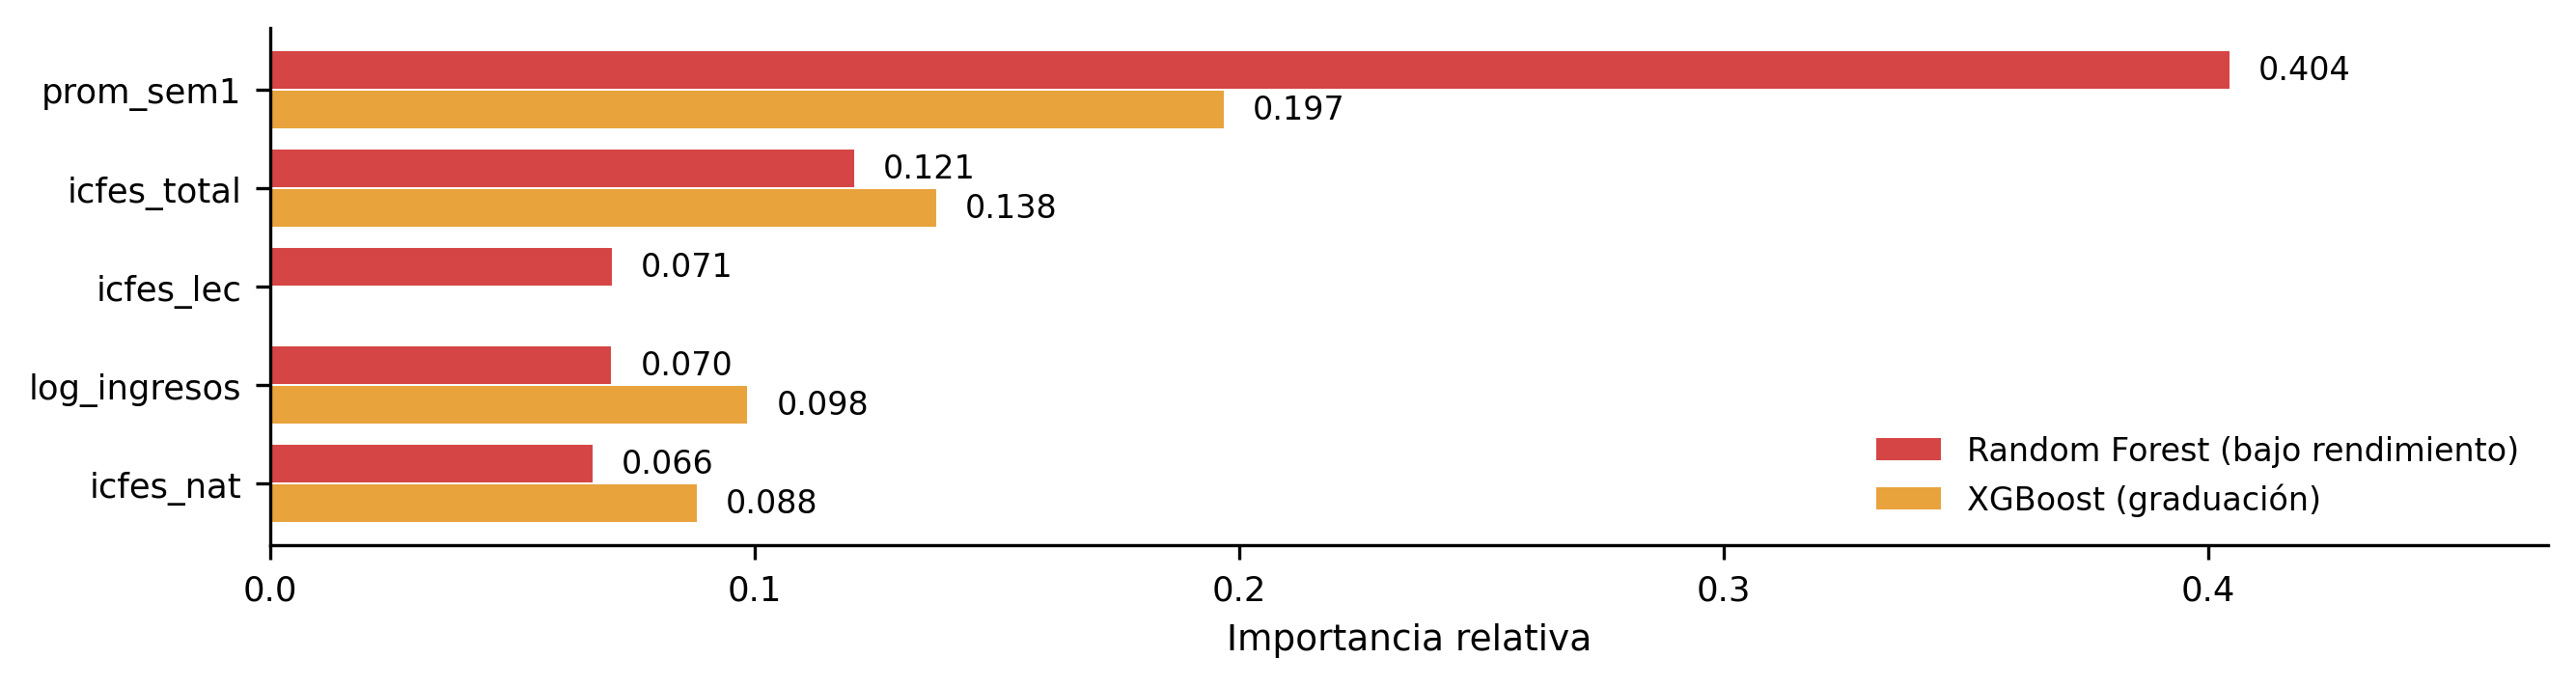
\includegraphics[width=\textwidth]{figuras/fig5_importancia_variables.png}
\caption{Importancia de las cinco variables principales en cada modelo
ganador.}\label{fig:importancia}
\end{figure}
 
\begin{table}[!ht]
\centering
\caption{Comparativa de modelos en validación cruzada de cinco pliegues
($N=90$).}\label{tab:comparativa}
\resizebox{\textwidth}{!}{
\begin{tabular}{llcccccc}
\toprule
\textbf{Objetivo} & \textbf{Modelo} & \textbf{Exhaust.}
& \textbf{Precisión} & \textbf{F1-mac} & \textbf{AUC}
& \textbf{MCC} & \textbf{Exactitud} \\
\midrule
\multirow{3}{*}{Bajo rendimiento ($u$=0,29)}
& Decision Tree & 0,632 & \textbf{0,667} & \textbf{0,702}
  & 0,702 & \textbf{0,404} & \textbf{0,711} \\
& \textbf{Random Forest} $\checkmark$ & \textbf{0,816} & 0,484
  & 0,548 & 0,752 & 0,197 & 0,556 \\
& XGBoost & 0,737 & 0,596 & 0,677 & \textbf{0,776}
  & 0,367 & 0,678 \\
\midrule
\multirow{3}{*}{Graduación ($u$=0,50)}
& Decision Tree & \textbf{0,686} & 0,686 & 0,743
  & 0,728 & 0,486 & 0,756 \\
& Random Forest & 0,657 & \textbf{0,821} & \textbf{0,792}
  & 0,844 & \textbf{0,596} & \textbf{0,811} \\
& \textbf{XGBoost} $\checkmark$ & 0,600 & 0,808 & 0,764
  & \textbf{0,853} & 0,548 & 0,789 \\
\bottomrule
\end{tabular}
}
\end{table}
 
Entre los factores explorados, la comparación del promedio entre
hombres y mujeres no evidenció diferencias significativas (U de
Mann-Whitney, $p=0{,}246$)~\cite{guerrero2024}; tampoco se identificó
correlación entre el nivel educativo de los padres y el promedio
(Spearman, $p>0{,}6$), ni asociación entre repitencia escolar previa y
bajo rendimiento ($\chi^{2}$, $p=0{,}215$). Estos resultados negativos, condicionados por
el tamaño de los subgrupos, son consistentes con la dominancia del
desempeño académico temprano que evidencia la Fig.~\ref{fig:importancia}.
 
 
\begin{figure}[!ht]
\centering
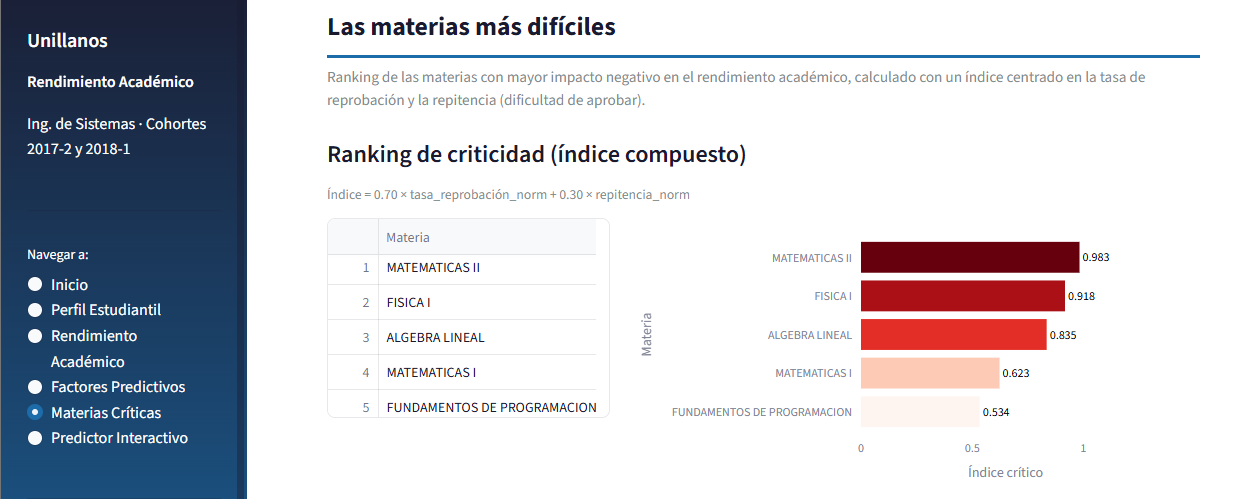
\includegraphics[width=\textwidth]{figuras/fig8_app_criticidad.png}
\caption{Aplicación en Streamlit: índice de criticidad de las cinco
asignaturas con mayor valor.}\label{fig:materias}
\end{figure}
 
Las cinco asignaturas de mayor índice de criticidad fueron
Matemáticas~II, Física~I, Álgebra Lineal, Matemáticas~I y Fundamentos
de Programación (Fig.~\ref{fig:materias}), todas ellas de los primeros
semestres del plan de estudios. 
 
 
%  4. CONCLUSIONES
\section{Conclusiones}
 
De los tres algoritmos evaluados, \textit{Random Forest} resultó el más adecuado
para predecir el bajo rendimiento (exhaustividad 0,816 con umbral
0,29), mientras que \textit{XGBoost} obtuvo el mayor AUC en graduación (0,853);
ninguno dominó ambos objetivos. En los dos
modelos el promedio del primer semestre fue la variable dominante, lo
que permite activar alertas tempranas al cierre del primer periodo; las
variables sociodemográficas y familiares no mostraron diferencias ni
asociaciones significativas en esta población. Las cinco asignaturas de
mayor criticidad se concentran en los primeros semestres, lo que
habilita intervenciones focalizadas en el mismo periodo en que el
modelo emite su primera alerta.
 
Como trabajo futuro se extenderá el análisis a los otros programas de la
Facultad de Ciencias Básicas e Ingeniería con una variable objetivo multiclase de trayectoria y diseño longitudinal por corte semestral.
 
\subsubsection{Agradecimientos.} Los autores agradecen al proyecto
DGI/Unillanos C07-02-2026-027.
 
%  REFERENCIAS (formato IEEE)
\begin{thebibliography}{8}
\setlength{\itemsep}{0pt}
\small
 
\bibitem{lee2023}
Laboratorio de Economía de la Educación, ``Deserción en la educación
superior en Colombia,'' Informe de análisis estadístico No.~74,
Pontificia Universidad Javeriana, Bogotá, Colombia, 2023.
 
\bibitem{romero2010}
C. Romero and S. Ventura, ``Educational data mining: A review of the
state of the art,'' \emph{IEEE Trans. Syst., Man, Cybern. C},
vol.~40, no.~6, pp.~601--618, 2010.
 
\bibitem{shahiri2015}
A. M. Shahiri, W. Husain, and N. A. Rashid, ``A review on predicting
student's performance using data mining techniques,''
\emph{Procedia Comput. Sci.}, vol.~72, pp.~414--422, 2015.
 
\bibitem{pipino2002}
L. L. Pipino, Y. W. Lee, and R. Y. Wang, ``Data quality assessment,''
\emph{Commun. ACM}, vol.~45, no.~4, pp.~211--218, 2002.
 
\bibitem{wirth2000}
R. Wirth and J. Hipp, ``CRISP-DM: Towards a standard process model for
data mining,'' in \emph{Proc. 4th Int. Conf. Practical Applications of
Knowledge Discovery and Data Mining}, 2000, pp.~29--39.
 
\bibitem{breiman1984}
L. Breiman, J. H. Friedman, R. A. Olshen, and C. J. Stone,
\emph{Classification and Regression Trees}. Belmont, CA, USA:
Wadsworth, 1984.
 
\bibitem{guerrero2024}
S. C. Guerrero and R. L. Espejo, ``Deserción universitaria: estudio
comparativo entre Colombia y España desde la perspectiva de género,''
\emph{Formación Universitaria}, vol.~17, no.~2, pp.~101--112, 2024.
 
\bibitem{fawcett2006}
T. Fawcett, ``An introduction to ROC analysis,''
\emph{Pattern Recognit. Lett.}, vol.~27, no.~8, pp.~861--874, 2006.
 
\end{thebibliography}
 
\end{document}